\begin{frame}
	\frametitle{Detección de Keypoints}
	
	\note{https://youtu.be/ebMyBbkkHWk}
	
	\footnotesize
	Propiedades deseables para SLAM / SfM:
	\begin{itemize}
		\item Alta repetitibilidad
		\item Alta precisión
		\item Robustez
		\item Invarianza (luminosidad, puntos de vista, etc)
		\item Computacionalmente eficientes
		\item Algunos detectores: HARRIS, SIFT, SURF, Shi-Tomasi, FAST, ORB, BRISK
	\end{itemize}

	
	\begin{figure}
		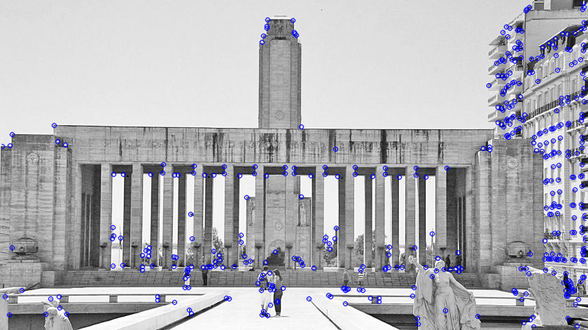
\includegraphics[width=0.5\textwidth]{./images/keypoints_fast}
		\caption{Keypoints FAST}
	\end{figure}

\end{frame}


\begin{frame}
	\frametitle{Matcheo de keypoints}
	\footnotesize
	Propiedades deseables del matcheo de keypoints para SLAM / SfM:
	\begin{itemize}
		\item Alto recall
		\item precisión
		\item Robustez
		\item Computacionalmente eficientes
		\item Posibles enfoques: patches o descriptores
	\end{itemize}
	
	\begin{figure}
		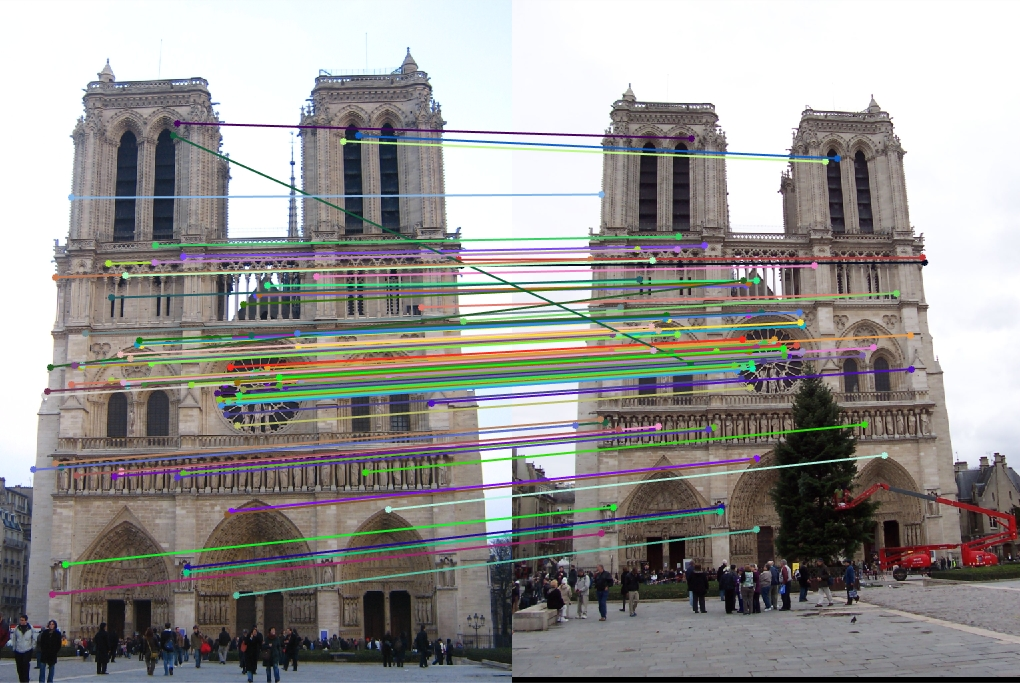
\includegraphics[width=0.4\textwidth]{./images/matching_notredam.jpg}
		\caption{Keypoints Harris + Descriptor SIFT}
	\end{figure}
	\note{Imagen extraida de https://www.cc.gatech.edu/classes/AY2016/cs4476_fall/results/proj2/html/cpolack6/index.html}
\end{frame}

\begin{frame}
	\frametitle{Precision - Recall}
	\footnotesize
	
	\note{https://upload.wikimedia.org/wikipedia/commons/2/26/Precisionrecall.svg}
	
	\begin{figure}
		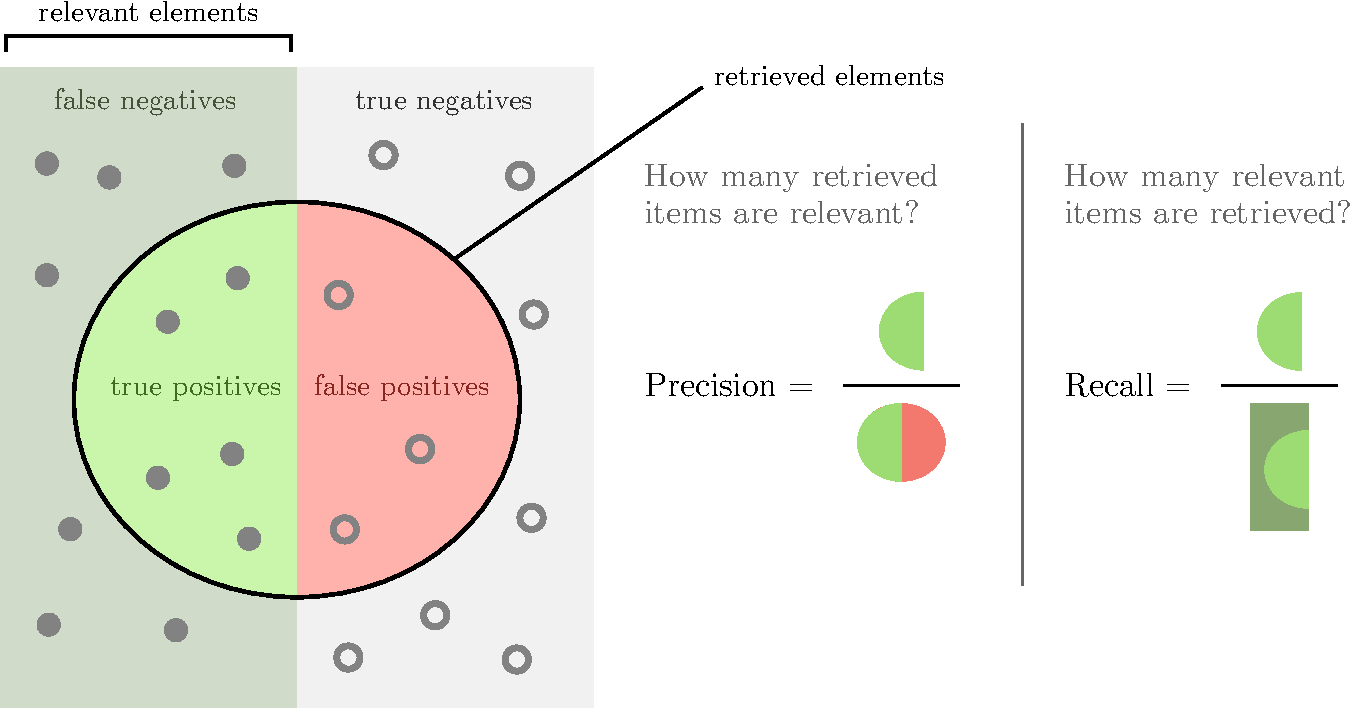
\includegraphics[width=0.25\textwidth]{./images/precision_recall.pdf}
	\end{figure}
\end{frame}

\begin{frame}
	\frametitle{Desciptores de features Locales}
	\footnotesize
	
	Propiedades deseables para SLAM / SfM: distinguibles, robustos, invariantes
	\begin{itemize}
		\item Extraer firmas sobre regiones de la imagen ejemplos:
		\begin{itemize}
			\item Histogramas sobre gradientes de la imagen (SIFT)
			\item Histogramas sobre respuestas Haar-wavelet (SURF)
			\item Patrones binarios (BRIEF, BRISK, FREAK, ORB)
			\item Descriptores basados en aprendizaje
		\end{itemize}
		\item Invariante rotación: Alineado con la orientación dominante de la región local
		\item Invariante a escala: Adaptar la región descripta a la escala de keypoint
	\end{itemize}
	
\end{frame}

\begin{frame}
	\frametitle{Matcheo de keypoints}
	\footnotesize
	
\end{frame}

\begin{frame}
	\frametitle{Matcheo de keypoints}
	\footnotesize
	
\end{frame}

\begin{frame}
	\frametitle{Matcheo de keypoints}
	\footnotesize
	
\end{frame}

\begin{frame}
	\frametitle{Matcheo de keypoints}
	\footnotesize
	
\end{frame}

\begin{frame}
	\frametitle{Matcheo de keypoints}
	\footnotesize
	
\end{frame}

\begin{frame}
	\frametitle{Matcheo de keypoints}
	\footnotesize
	
\end{frame}

\begin{frame}
	\frametitle{Matcheo de keypoints}
	\footnotesize
	
\end{frame}

\begin{frame}
	\frametitle{Matcheo de keypoints}
	\footnotesize
	
\end{frame}

\begin{frame}
	\frametitle{Matcheo de keypoints}
	\footnotesize
	
\end{frame}

\begin{frame}
	\frametitle{Matcheo de keypoints}
	\footnotesize
	
\end{frame}

\begin{frame}
	\frametitle{Matcheo de keypoints}
	\footnotesize
	
\end{frame}

\begin{frame}
	\frametitle{Matcheo de keypoints}
	\footnotesize
	
\end{frame}


